Our robot Dora is created using the differential platform Pioneer 3D-X and central supporting construction for sensors and a laptop, see Fig~\ref{fig:Dora}. 
In last year, Dora was equipped with 2 laser rangefinders and 1 depth camera, which were used to ensure safe navigation 
and people detection. 
This year, we are going to significantly improve Dora's hardware in order to provide more support for:
\begin{itemize}
\item \textit{human robot interaction} - Dora's speech understanding and speech reproduction were strongly limited to the used laptop last year. 
We are going to extend Dora by mounting a microphone and a speaker on her. Additionally, we are going to improve her appearance to be more user-friendly. 
\item \textit{safe and robust navigation} - We are investigating usage of Pioneer's sonar to detect small objects. 
Moreover, Pioneer's bumpers will be used to stop the robot when an object is hit. 
\item \textit{object recognition} - another depth camera with short range is added to allow detection of small household objects.
\end{itemize}
 
\begin{figure}[!htb]
\centering
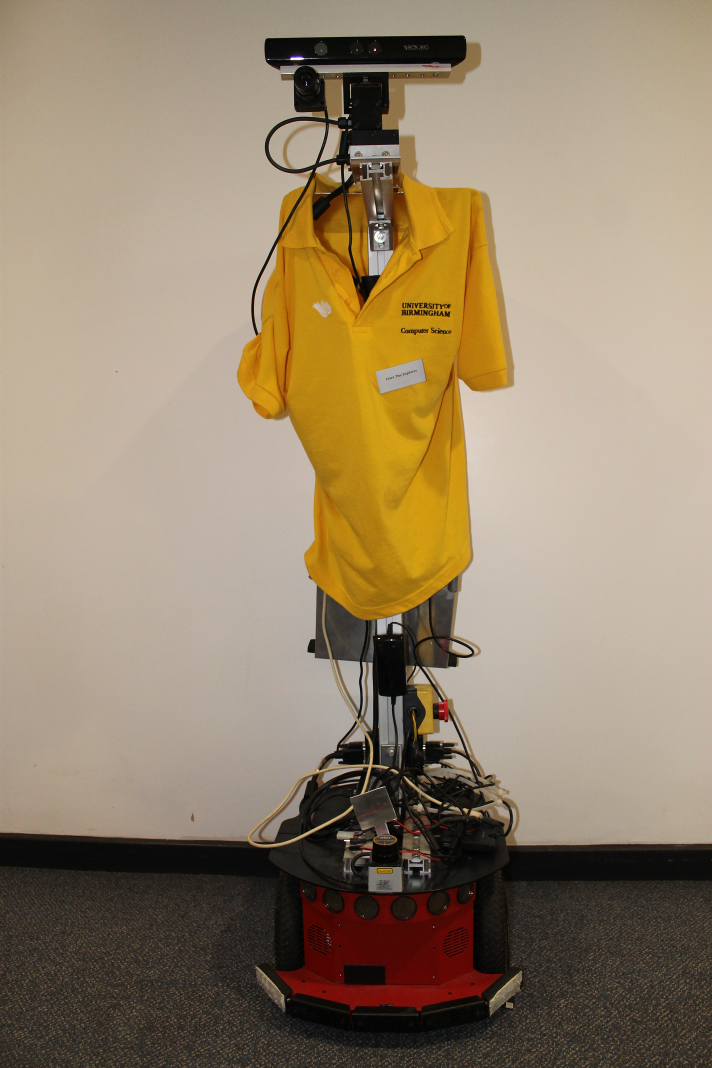
\includegraphics[width=2.in]{dora_new.png}
\caption{Dora is an extended Pioneer 3D-X robot with sensors such as a laser range finder, depth camera and a laptop mounted on top.}
\label{fig:dora}
\end{figure}  


